
\chapter{Demostración de la Peligrosidad del Modo ECB}

\section{Fundamento teórico: El problema del modo ECB}

El modo ECB (\textit{Electronic Codebook}) es uno de los modos de operación más simples e inseguros. Su funcionamiento es:

\begin{equation}
C_i = E(K, P_i)
\end{equation}

Donde cada bloque de texto plano $P_i$ se cifra independientemente con la misma clave $K$.

\subsection{Problemas de seguridad}

\begin{enumerate}
    \item \textbf{Determinismo:} Bloques idénticos producen criptogramas idénticos.
    \item \textbf{Revelación de patrones:} Patrones que se revelan en el cifrado.
    \item \textbf{Análisis de frecuencia:} Posible análisis estadístico.
\end{enumerate}

\section{Experimento: Cifrado de imágenes}

\subsection{Procedimiento}

Se utilizó una imagen del logo de kali linux con colores sólidos para maximizar 
la visibilidad de los patrones. El proceso fue:

\begin{enumerate}
    \item Conversión de la imagen a formato PGM
    \item Separación de cabecera y datos binarios
    \item Cifrado de los datos con AES-256-ECB
    \item Reconstrucción de la imagen cifrada
    \item Conversión de vuelta al formato original
    \item Comparación con modo CBC
\end{enumerate}

\subsection{Comandos utilizados}

\begin{lstlisting}[caption=Cifrado ECB de imágenes]
# Convertir a PGM
convert imagen.png imagen.pgm

# Separar cabecera y datos
head -n 3 imagen.pgm > cabecera.txt
tail -n +4 imagen.pgm > datos.bin

# Cifrado ECB (INSEGURO)
openssl enc -aes-256-ecb -in datos.bin -out datos_ecb.bin \
    -K 0123456789ABCDEF... -nosalt

# Reconstruir y convertir
cat cabecera.txt datos_ecb.bin > imagen_cifrada.pgm
convert imagen_cifrada.pgm imagen_cifrada.png
\end{lstlisting}

\subsection{Comparación de modos}
Imagen original:
\begin{center}
    
\includegraphics[width=0.4\textwidth]{imagenes/ImagenesEncriptadas/kalili.png}
\end{center}

\begin{table}[H]
    \centering
    \caption{Comparación de modos de operación}
    \begin{tabularx}{\textwidth}{l|p{3cm}|p{3cm}}
        \toprule
        \textbf{Modo} & \textbf{Resultado} & \textbf{Seguridad} \\
        \midrule
        ECB 3DES & \textit{Se distinguen patrones de la imagen original} & 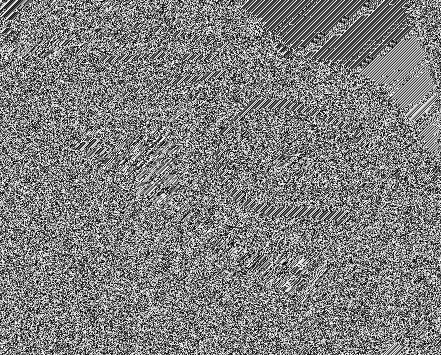
\includegraphics[width=0.4\textwidth]{imagenes/ImagenesEncriptadas/imagen_cifrada_des_ecb.png}\\
        CBC & \textit{Imagen completamente aleatoria} & 
\includegraphics[width=0.4\textwidth]{imagenes/ImagenesEncriptadas/imagen_cifrada_cbc.png} \\
        \bottomrule
    \end{tabularx}
\end{table}

\section{Resultados obtenidos}

\subsection{Imágenes generadas}

Se generaron las siguientes imágenes:

\begin{itemize}[label=\textbullet]
    \item \textbf{ECB con AES-256:} Los patrones originales son vagamente visibles.
    \item \textbf{ECB con 3DES:} Patrones muy pronunciados debido a bloques de 64 bits.
    \item \textbf{CBC con AES-256:} Imagen completamente aleatoria.
\end{itemize}

\section{Conclusiones sobre seguridad}
Utilizar el modo ECB para cifrar datos sensibles es extremadamente peligroso, especialmente
con datos que contienen patrones repetitivos, como imágenes, y aún más peligroso si se
 utilizan algoritmos con bloques pequeños como 3DES.\@ En contraste, modos como CBC ofrecen 
 una seguridad mucho mayor al introducir aleatoriedad y dependencia entre bloques, 
 evitando la revelación de patrones y protegiendo la confidencialidad de los datos.